% arara: xelatex: {shell: yes}
%% arara: biber
%% arara: xelatex: {shell: yes}
%% arara: xelatex: {shell: yes}


% Здесь мы держим компромисс между красотой и легкостью включения новых людей в процесс создания.
% Поэтому не используем пакеты, которые требуют возни с установкой и настройкой.
% Например, используем listings вместо minted.
% Пакет minted требует настроенного питона и связки латех-питон. 
% Вместо arara используем классический latexmk. 





%!TeX cleanPatterns = $OUTDIR/$JOB!($OUTEXT|.synctex.gz|.tex|.pdf), /$OUTDIR/_minted-$JOB/
\documentclass[12pt, a4paper]{article}

% utf8 is the preferred encoding

 % this magic is to solve problem that appeared after update of texlive 2018 to texlive 2020
 % https://tex.stackexchange.com/questions/511341/the-error-occurred-after-the-last-update
\makeatletter
\def\nobreak{\penalty\@M}
\makeatother

\usepackage{comment}

\usepackage{fontspec} % что-то про шрифты? % нужно ли загружать?

\usepackage{polyglossia} % русификация xelatex
\usepackage{csquotes}
\usepackage{wrapfig} % обтекание картинок
\usepackage{xparse} % для прикольных вероятностей


\setmainlanguage{russian}

% download "Linux Libertine" fonts:
% http://www.linuxlibertine.org/index.php?id=91&L=1
\setmainfont{Linux Libertine O} % or Helvetica, Arial, Cambria
% why do we need \newfontfamily:
% http://tex.stackexchange.com/questions/91507/
\newfontfamily{\cyrillicfonttt}{Linux Libertine O}

\newfontfamily\arabicfont[Script=Arabic]{Scheherazade New}


\usepackage{etoolbox} % provides \AtEndPreamble
% etoolbox causes wrong behavior of tocbasic
\AtEndPreamble{ % ради арабского написания Абу ибн-Сина
  \usepackage{arabxetex} 
 \let\textarabic\relax 
 \let\Arabic\relax 
\setotherlanguages{arabic, english}
}
% комбо из:
% https://tex.stackexchange.com/questions/501897
% https://tex.stackexchange.com/questions/392175/

\usepackage[nonewpage]{imakeidx} 
%\indexsetup{level=\section}
\indexsetup{level=\section,toclevel=section,noclearpage}
\makeindex[intoc,title={Модные хэштэги}] % [title=Модные хэштэги, intoc]
% TODO: лишняя пустая страница в printindex

\usepackage{etex} % расширение классического tex
% в частности позволяет подгружать гораздо больше пакетов, чем мы и займёмся далее

\usepackage{verbatim} % для многострочных комментариев
\usepackage{makeidx} % для создания предметных указателей

\usepackage{setspace}
\usepackage{amsmath, amsfonts, amssymb, amsthm}
\usepackage{mathrsfs} % sudo yum install texlive-rsfs
\usepackage{dsfont} % sudo yum install texlive-doublestroke
\usepackage{array, multicol, multirow, bigstrut} % sudo yum install texlive-multirow
\usepackage{indentfirst} % установка отступа в первом абзаце главы


\usepackage{bm}
\usepackage{bbm} % шрифт с двойными буквами
%\usepackage[perpage]{footmisc}

\usepackage{dcolumn} % центрирование по разделителю для apsrtable

% создание гиперссылок в pdf
\usepackage[unicode, colorlinks=true, urlcolor=blue, hyperindex, breaklinks]{hyperref}


\usepackage{microtype} % свешиваем пунктуацию
% теперь знаки пунктуации могут вылезать за правую границу текста, при этом текст выглядит ровнее


\usepackage{textcomp}  % Чтобы в формулах можно было русские буквы писать через \text{}

% размер листа бумаги
%\usepackage[paperwidth=145mm,paperheight=215mm,
%height=182mm,width=113mm,top=20mm,includefoot]%{geometry}
\usepackage[paper=a4paper, top=15mm, bottom=13.5mm, left=16.5mm, right=13.5mm, includefoot]{geometry}

\usepackage{xcolor}
\usepackage{framed} % для рамок и черты слева от минитеории, \leftbar

% \usepackage{float, longtable}
\usepackage{soulutf8}

\usepackage{enumitem} % дополнительные плюшки для списков
%  например \begin{enumerate}[resume] позволяет продолжить нумерацию в новом списке

\usepackage{mathtools}
\usepackage{cancel, xspace} % sudo yum install texlive-cancel


\usepackage{numprint} % sudo yum install texlive-numprint
\npthousandsep{,}\npthousandthpartsep{}\npdecimalsign{.}


% \usepackage{subfigure} % для создания нескольких рисунков внутри одного

\usepackage{tikz, pgfplots} % язык для рисования графики из latex'a
\pgfplotsset{compat=1.16}
\usetikzlibrary{trees} % tikz-прибамбас для рисовки деревьев
\usepackage{tikz-qtree} % альтернативный tikz-прибамбас для рисовки деревьев
\usepackage{tkz-graph} % by dp for making prob trees
\usetikzlibrary{arrows} % tikz-прибамбас для рисовки стрелочек подлиннее

\usepackage{todonotes} % для вставки в документ заметок о том, что осталось сделать
% \todo{Здесь надо коэффициенты исправить}
% \missingfigure{Здесь будет Последний день Помпеи}
% \listoftodos — печатает все поставленные \todo'шки



\usepackage{booktabs} %  красивые таблицы
% заповеди из докупентации:
% 1. Не используйте вертикальные линни
% 2. Не используйте двойные линии
% 3. Единицы измерения - в шапку таблицы
% 4. Не сокращайте .1 вместо 0.1
% 5. Повторяющееся значение повторяйте, а не говорите "то же"

\usepackage{physics}

\usepackage{listings}
\lstset{%
basicstyle=\fontfamily{lmtt}\bfseries,
keywordstyle=\fontfamily{lmtt}\bfseries
}

\usepackage{answers}

\newenvironment{rus}{}{} % environment just prints the text
\newenvironment{eng}{}{}
\excludecomment{eng}



\usepackage[bibencoding=auto, backend=biber, sorting=none, style=alphabetic]{biblatex}

\addbibresource{probability_pro.bib}

\setcounter{tocdepth}{1} % в оглавление оставляем уровень 1

\usepackage[titles]{tocloft} % альтернатива tocbasic для настройки toc
% если нужен subfigure, то у tocloft можно добавить опцию subfigure
\renewcommand{\cftbeforesecskip}{0.7pt} % поправка интервала между строками для section в toc
\renewcommand{\cftsecdotsep}{\cftdotsep} % добавляем точечки

\AddEnumerateCounter{\asbuk}{\russian@alph}{щ} % для списков с русскими буквами
\setlist[enumerate, 1]{label=\asbuk*),ref=\asbuk*} % цифра рядом с enumerate = уровень нумерации



%%%%%%%%%%%%%%%%%%%%%%%  ПАРАМЕТРЫ  %%%%%%%%%%%%%%%%%%%%%%%%%%%%%%%%%%
\setstretch{1}                          % Межстрочный интервал
\flushbottom                            % Эта команда заставляет LaTeX чуть растягивать строки, чтобы получить идеально прямоугольную страницу
\righthyphenmin=2                       % Разрешение переноса двух и более символов
%\pagestyle{plain}                       % Нумерация страниц снизу по центру.
\widowpenalty=300                     % Небольшое наказание за вдовствующую строку (одна строка абзаца на этой странице, остальное — на следующей)
\clubpenalty=3000                     % Приличное наказание за сиротствующую строку (омерзительно висящая одинокая строка в начале страницы)
\setlength{\parindent}{1.5em}           % Красная строка.
%\captiondelim{. }
\setlength{\topsep}{0pt}
\emergencystretch=2em

% делаем короче интервал в списках
\setlength{\itemsep}{0pt}
\setlength{\parskip}{0pt}
\setlength{\parsep}{0pt}



\DeclareMathOperator{\card}{card}
\DeclareMathOperator{\sign}{sign}
\DeclareMathOperator{\sgn}{sign}

\DeclareMathOperator*{\argmin}{arg\,min}
\DeclareMathOperator*{\amn}{arg\,min}
\DeclareMathOperator*{\amx}{arg\,max}


\DeclareMathOperator{\Corr}{Corr}
\DeclareMathOperator{\sCorr}{sCorr}
\DeclareMathOperator{\sCov}{sCov}
\DeclareMathOperator{\sVar}{sVar}

%\DeclareMathOperator{\Cov}{Cov}
%\DeclareMathOperator{\Var}{Var}

\DeclareMathOperator*{\plim}{plim}
\DeclareMathOperator{\MSE}{MSE}
\DeclareMathOperator{\softmax}{softmax}
\DeclareMathOperator{\Med}{Med}


\DeclareMathOperator{\col}{col}
\DeclareMathOperator{\row}{row}


\let\P\relax
\DeclareMathOperator{\P}{\mathbb{P}}

% \newcommand{\P}{\mathbb{P}}



\newcommand{\oP}{o_{\operatorname{P}}} % вероятностное о-малое




\newcommand{\e}{\varepsilon}

\newcommand{\cN}{\mathcal{N}}

% вместо горизонтальной делаем косую черточку в нестрогих неравенствах
\renewcommand{\le}{\leqslant}
\renewcommand{\ge}{\geqslant}
\renewcommand{\leq}{\leqslant}
\renewcommand{\geq}{\geqslant}


\newcommand{\wv}{\textrm{word2vec}}
\newcommand{\hVar}{\widehat{\Var}}
\newcommand{\hCorr}{\widehat{\Corr}}
\newcommand{\hCov}{\widehat{\Cov}}


\newcommand{\PP}{\mathbb{P}}
\newcommand{\QQ}{\mathbb{Q}}
\newcommand{\RR}{\mathbb{R}}
\newcommand{\NN}{\mathbb{N}}
\newcommand{\ZZ}{\mathbb{Z}}
\newcommand{\cF}{\mathcal{F}}
\newcommand{\cB}{\mathcal{B}}
\newcommand{\cA}{\mathcal{A}}
\newcommand{\cH}{\mathcal{H}}


% dot of variable size, from
% https://tex.stackexchange.com/questions/389238/is-there-a-black-dot-symbol-that-i-can-use
\newcommand\vardot[1][.4]{\mathbin{\vcenter{\hbox{\scalebox{#1}{$\bullet$}}}}}
% dot above equality sign for Newton style
%\renewcommand{\doteq}{\mathrel{\overset{\vardot}{=}}}
\renewcommand{\doteq}{\mathrel{\overset{\lim}{=}}}



% from Blitzstein


\newcommand{\dBern}{\mathrm{Bern}}
\newcommand{\dPois}{\mathrm{Pois}}
\newcommand{\dBin}{\mathrm{Bin}}
\newcommand{\dMult}{\mathrm{Mult}}
\newcommand{\dGeom}{\mathrm{Geom}}
\newcommand{\dNHGeom}{\mathrm{NHGeom}}
\newcommand{\dHGeom}{\mathrm{HGeom}}
\newcommand{\dDUnif}{\mathrm{DUnif}}
\newcommand{\dFS}{\mathrm{FS}}
\newcommand{\dNBin}{\mathrm{NBin}}

\newcommand{\dTri}{\mathrm{Triangle}}
\newcommand{\dUnif}{\mathrm{Unif}}
\newcommand{\dU}{\mathrm{U}}
\newcommand{\dCauchy}{\mathrm{Cauchy}}
\newcommand{\dN}{\mathcal{N}}
\newcommand{\dLN}{\mathcal{LN}}
\newcommand{\dExpo}{\mathrm{Expo}} % o is probably great to avoid confusion with exp function
\newcommand{\dExp}{\dExpo}
\newcommand{\dBeta}{\mathrm{Beta}}
\newcommand{\dGamma}{\mathrm{Gamma}}
\newcommand{\dWei}{\mathrm{Wei}}
\newcommand{\dLogistic}{\mathrm{Logistic}}
\newcommand{\dRayleigh}{\mathrm{Rayleigh}}
\newcommand{\dPareto}{\mathrm{Pareto}}


\newcommand{\addtag}[1]{\index{#1}}

\DeclareMathOperator{\Convex}{Convex}
\DeclareMathOperator{\Hull}{Hull}
\DeclareMathOperator{\hull}{\Hull}
\DeclareMathOperator{\Span}{Span}
\DeclareMathOperator{\cone}{Cone}




% hack from
% https://tex.stackexchange.com/questions/14501/making-footnote-work-in-leftbar-environment/
% does not work with hyperref?
% \input{footnote-in-leftbar.tex}

\title{Заметки к семинарам по методам оптимальных решений}
\author{\url{https://github.com/bdemeshev/optimal-solution-pro} \\
зеркало: \url{https://gitlab.com/bdemeshev/optimal-solution-pro}}
\date{\today \\ 
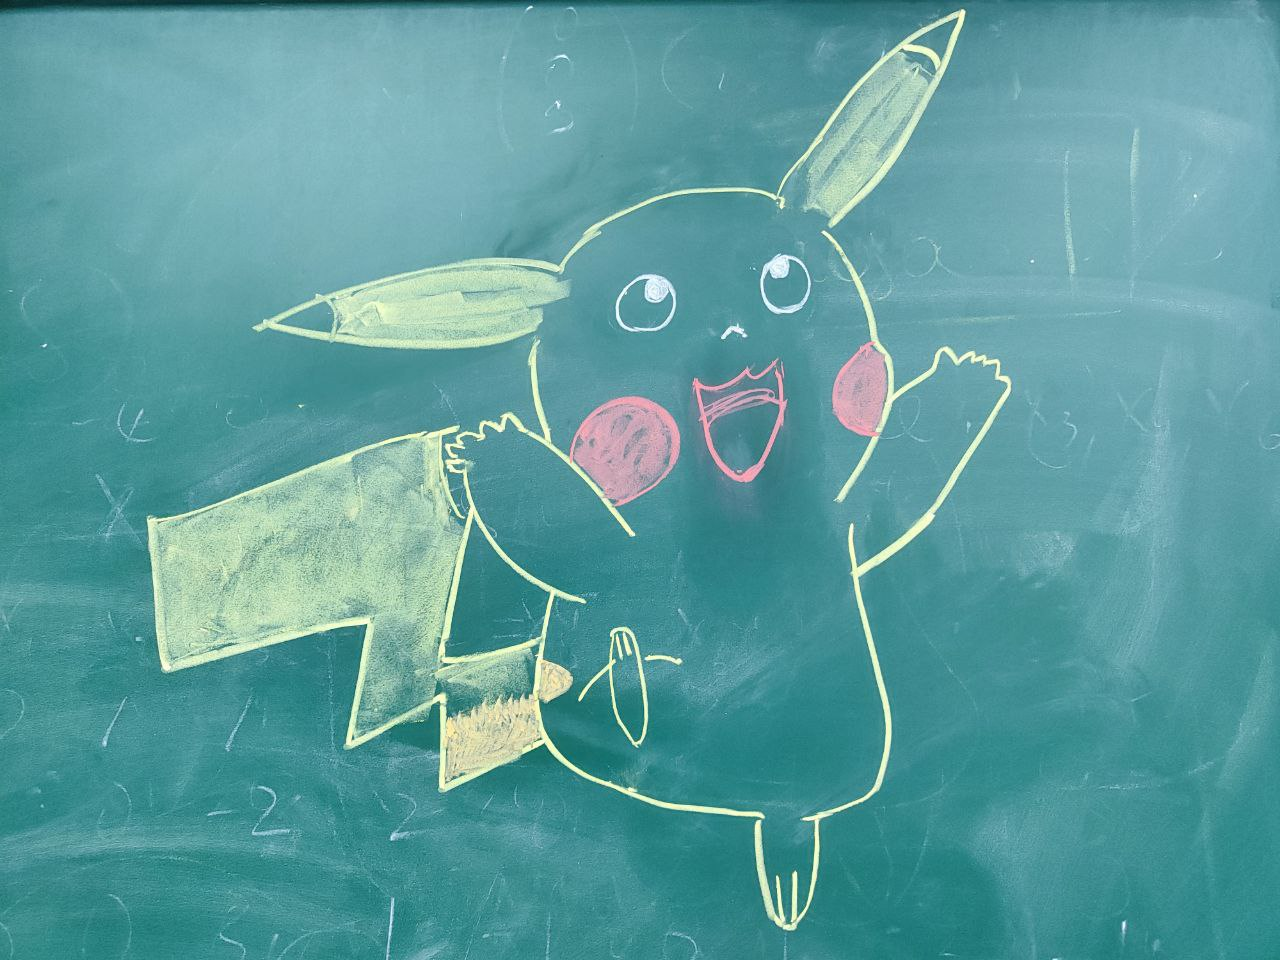
\includegraphics[height=10cm]{picachu.jpg}}


%\newtheorem{problem}{Задача}
%\numberwithin{problem}{section}

\Newassociation{sol}{solution}{solution_file}
% sol — имя окружения внутри задач
% solution — имя окружения внутри solution_file
% solution_file — имя файла в который будет идти запись решений
% можно изменить далее по ходу
\Opensolutionfile{solution_file}[all_solutions]
% в квадратных скобках фактическое имя файла



% магия для автоматических гиперссылок задача-решение
\newlist{myenum}{enumerate}{3}
% \newcounter{problem}[chapter] % нумерация задач внутри глав
\newcounter{problem}[section]

\newenvironment{problem}%
{%
\refstepcounter{problem}%
%  hyperlink to solution
     \hypertarget{problem:{\thesection.\theproblem}}{} % нумерация внутри глав
     % \hypertarget{problem:{\theproblem}}{}
     \Writetofile{solution_file}{\protect\hypertarget{soln:\thesection.\theproblem}{}}
     %\Writetofile{solution_file}{\protect\hypertarget{soln:\theproblem}{}}
     \begin{myenum}[label=\bfseries\protect\hyperlink{soln:\thesection.\theproblem}{\thesection.\theproblem},ref=\thesection.\theproblem]
     % \begin{myenum}[label=\bfseries\protect\hyperlink{soln:\theproblem}{\theproblem},ref=\theproblem]
     \item%
    }%
    {%
    \end{myenum}}
% для гиперссылок обратно надо переопределять окружение
% это происходит непосредственно перед подключением файла с решениями





\begin{document}

\maketitle % ставим сюда название, автора и время создания

% здесь нужна прикольная картинка

\newpage
\tableofcontents{}

\newpage

При везении подсказку, ответ или решение можно найти, кликнув по номеру задачи. 

% Если \url{github.com} не открывается, можно заменить его на \url{gitlab.com}.


\section{Картинки на плоскости}

\begin{leftbar}
\noindent
Линейная оболочка (linear span):
\[
  \Span(v_1, v_2, v_3) = \{x_1 v_1 + x_2 v_2 + x_3 v_3 \mid x_1 \in \RR, x_2 \in \RR, x_3 \in \RR \}
\]
Конус (cone):
\[
  \cone(v_1, v_2, v_3) = \{x_1 v_1 + x_2 v_2 + x_3 v_3 \mid x_1 \geq 0, x_2 \geq 0, x_3 \geq 0 \}
\]
Выпуклая линейная оболочка (convex linear hull):
\[
  \Hull(v_1, v_2, v_3) = \Convex(v_1, v_2, v_3) = \left\{x_1 v_1 + x_2 v_2 + x_3 v_3 \mid x_1 \geq 0, x_2 \geq 0, x_3 \geq 0, \sum x_i = 1 \right\}
\]
\end{leftbar}


\begin{problem}
  Рассмотрим точки на плоскости, $A = (0, 0)$, $B = (5, 3)$ и $C = (5, -3)$.
  
  \begin{enumerate}
    \item Нарисуйте точки $0.5 B + 0.5 C$, $0.9 A + 0.1 B$, $3 B - 2 C$.
    \item Нарисуйте точки $\frac{1}{3}A + \frac{1}{3}B + \frac{1}{3}C$, $0.1 A + 0.45 B + 0.45 C$, $0.9A + 0.05B + 0.05C$.
  \end{enumerate}
  
  \begin{sol}
  
  \end{sol}
  \end{problem}
  


\begin{problem}
Рассмотрим точки на плоскости, $A = (1, 2)$, $B = (3, 4)$ и $C = (5, 1)$.

\begin{enumerate}
  \item Нарисуйте $\hull(A, B)$, $\hull(A, B, C)$.
  \item Нарисуйте $\cone(A)$, $\cone(A, B)$, $\cone(A, B, C)$.
  \item Нарисуйте $\Span(A)$, $\Span(A, B)$.
  \item Нарисуйте $A + \Span(B)$, $\cone(A) + \cone(B)$.
  \item Нарисуйте $\hull(A, B) + \cone(C)$, $\hull(A) + \cone(B, C)$, $\hull(A, C) + \cone(B, C)$.
\end{enumerate}

\begin{sol}

\end{sol}
\end{problem}


\begin{problem}
Рассмотрим точки на плоскости $A = (1, 2)$, $B = (5, 2)$, $C = (1, 4)$, $D = (5, 4)$.
\begin{enumerate}
  \item Запишите $E = (1, 3)$ как выпуклую линейную комбинацию точек $A$, $B$, $C$ и $D$.
  \item Запишите $F = (3, 3)$ как выпуклую линейную комбинацию точек $A$, $B$, $C$ и $D$ всеми возможными способами.
  \item Можно ли записать $G = (6, 3)$ как выпуклую линейную комбинацию точек $A$, $B$, $C$ и $D$?
  \item Сколькими способами можно записать $H = (4, 3)$ как выпуклую линейную комбинацию $A$, $B$, $C$ и $D$?
  \item Сколькими способами можно записать $I = (4, 3)$ как выпуклую линейную комбинацию $A$, $B$ и $D$? 
  \item Сколькими способами можно записать $J = (4, 2)$ как выпуклую линейную комбинацию $A$, $B$, $C$ и $D$?
  \item Сколькими способами можно записать $K = (4, 2)$ как выпуклую линейную комбинацию $A$, $C$ и $D$?
\end{enumerate}

\begin{sol}
\begin{enumerate}
  \item $E = 0.5 A + 0B +  0.5 C + 0D$
  \item Например, $F = 0A + 0.5B + 0.5 C + 0D = 0.5A + 0B + 0C + 0.5D = 0.25A + 0.25B + 0.25C + 0.25D$.
  Для нахождения всех способов надо решить систему:
  \[
  \alpha A + \beta B + \gamma C + \delta D = E \\
  \alpha  + \beta  + \gamma  + \delta  = 1
  \]
  \[
\left(\begin{array}{cccc|c}
    1 & 5 & 1& 5 & 3 \\
    2 & 2 & 4 & 4 & 3 \\
    1 & 1 & 1 & 1 & 1 
\end{array}\right)    \to \ldots \to 
\left(\begin{array}{cccc|c}
    0 & 1 & 0 & 1 & 1/2 \\
    0 & 0 & 1 & 1 & 1/2 \\
    1 & 0 & 0 & -1 & 0 
\end{array}\right)
\]
  Система имеет бесконечное количество решений.

  Все способы, $F = \alpha A + (0.5 - \alpha) B + (0.5 - \alpha)C + \alpha D$, где $\alpha \in [0;0.5]$.
  \item Нельзя, так как $G \notin \hull(A, B, C, D)$.
  \item Есть $\infty$ способов.
  \item Есть $1$ способ. Решаем систему уравнений $I = t_1 A + t_2 B + (1 - t_1 - t_2)D$. 
  Получаем, что $I = 0.25 A + 0.25 B + 0.5 D$.
  \item Есть $1$ способ, $J = 0.25 A + 0.75 B$.
  \item $0$
\end{enumerate}

\end{sol}
\end{problem}

\begin{problem}
\begin{enumerate}
  \item Нарисуйте семейство прямых $a x_1 + 5x_2 = 10$ на плоскости $(x_1, x_2)$.
  \item Нарисуйте семейство прямых $2 x_1 + x_2 = d$ на плоскости $(x_1, x_2)$.
\end{enumerate}
  
\begin{sol}
    
\end{sol}
\end{problem}
  





\section{Оптимизация на плоскости}

\begin{problem}
  
\begin{sol}
  
\end{sol}
\end{problem}
  
\subsection{Оптимизация на плоскости с параметром}



\begin{problem}
Решите задачу линейного программирования при всех значениях $c$:  
\begin{gather}
  cx_1 + x_2 \to \max \\
  2x_1 + 3x_2 \leq 6 \\
  x_1 \geq 0 \\
  x_2 \geq 0 
\end{gather}
\begin{sol}
\end{sol}
\end{problem}
  
\begin{problem}
  Решите задачу линейного программирования при всех значениях $a$:  
  \begin{gather}
    x_1 + 3x_2 \to \max \\
    2x_1 + ax_2 \leq 6 \\
    x_1 \geq 0 \\
    x_2 \geq 0 
  \end{gather}
  \begin{sol}
  \end{sol}
  \end{problem}
  



\section{Симплекс-метод}


\begin{leftbar}
  \noindent
  Решение $x$ системы $Ax = b$ называется \textit{допустимым}, если все $x_i \geq 0$. 

  \noindent
  Решение $x$ системы $Ax = b$ называется \textit{базисным}, если столбцы $\col_i A$ при $x_i \neq 0$ линейно независимы.
\end{leftbar}
  

\section*{Терминология}

\begin{problem}
    Рассмотрим систему уравнений
    \[
    \begin{cases}
      2x_1 + 3x_2 + x_3 = 8 \\
      x_1 - x_2 + x_4 = 9
    \end{cases}  
    \]
    Есть несколько векторов, $x_a = (0,0,0,0)$, $x_b=(0,0, 8, 9)$, $x_c = (1,0,6,8)$, $x_d=(1,-9,33, -1)$, $x_e=(0,-9,35,0)$.

    \begin{enumerate}
      \item Какие векторы являются решениями системы?
      \item Какие векторы являются базисными решениями системы?
      \item Какие векторы являются допустимыми решениями при условии, что все $x_i \geq 0$?
    \end{enumerate}
\begin{sol}

  \begin{tabular}{lccc}
  \toprule
    вектор & решение & базисное решение & допустимое решение \\
  \midrule
  $x_a = (0,0,0,0)$ & нет & нет & нет \\
  $x_b=(0,0, 8, 9)$ & да & да & да \\
  $x_c = (1,0,6,8)$ & да & нет & да \\
  $x_d=(1,-9,33, -1)$ & да & нет & нет \\
  $x_e=(0,-9,35,0)$ & да & да & нет \\
  \bottomrule
  \end{tabular}
    
\end{sol}
\end{problem}
  
\begin{problem}
  Рассмотрим систему уравнений
  \[
  \begin{cases}
    x_1 + 3x_2 + x_3 = 10 \\
    2x_1 + x_2 + x_4 = 11
  \end{cases}  
  \]
  Есть несколько векторов, $x_a = (1,2,3,4)$, $x_b=(0,0, 10, 11)$, $x_c = (1,0,9,9)$, $x_d=(6,-1,7, 0)$, $x_e=(0,11,-23,0)$.

  \begin{enumerate}
    \item Какие векторы являются решениями системы?
    \item Какие векторы являются базисными решениями системы?
    \item Какие векторы являются допустимыми решениями при условии, что все $x_i \geq 0$?
  \end{enumerate}
\begin{sol}
  \begin{tabular}{lccc}
    \toprule
      вектор & решение & базисное решение & допустимое решение \\
    \midrule
    $x_a = (1,2,3,4)$ & нет & нет & нет \\
    $x_b=(0,0, 10, 11)$ & да & да & да \\
    $x_c = (1,0,9,9)$ & да & нет & да \\
    $x_d=(6,-1,7, 0)$ & да & нет & нет \\
    $x_e=(0,11,-23,0)$ & да & да & нет \\
    \bottomrule
  \end{tabular}
\end{sol}
\end{problem}


\begin{problem}
  Рассмотрим систему ограничений в канонической форме:
  \[
  \begin{cases}
    2x_1 + 5x_2 + x_3 = 8 \\
    x_1 - 6x_2 + x_4 = 15 \\
    -x_1 + 2x_2 + x_5 = 11 \\
    x_1 \geq 0, x_2 \geq 0, x_3 \geq 0, x_4 \geq 0, x_5 \geq 0. 
  \end{cases}  
  \]
  \begin{enumerate}
    \item Найдите хотя бы одно базисное допустимое решение системы.
    \item Найдите все базисные допустимые решения системы.
  \end{enumerate}

\begin{sol}
  \begin{enumerate}
    \item $x = (0, 0, 8, 15, 11)$
    \item 
  \end{enumerate}
  
\end{sol}
\end{problem}


\begin{problem}
  Рассмотрим систему ограничений в канонической форме:
  \[
  \begin{cases}
    2x_1 + 5x_2 - x_3 = 8 \\
    x_1 - 6x_2 + x_4 = 15 \\
    -x_1 + 2x_2 + x_5 = 11 \\
    x_1 \geq 0, x_2 \geq 0, x_3 \geq 0, x_4 \geq 0, x_5 \geq 0. 
  \end{cases}  
  \]
  \begin{enumerate}
    \item Найдите хотя бы одно базисное допустимое решение системы.
    \item Найдите все базисные допустимые решения системы.
  \end{enumerate}


\begin{sol}
  \begin{enumerate}
    \item Решение $x = (0, 0, -8, 15, 11)$ является базисным и не является допустимым.
  Подойдёт, например, $x = (4, 0, 0, 11, 15)$.
  \item 
\end{enumerate}

\end{sol}
\end{problem}




\section*{Приятная стартовая точка}

\begin{problem}
  Рассмотрим задачу линейного программирования:
  \[
  \begin{cases}
    x_1 + x_2 \to \max \\
    x_1 + 3x_2 \leq 9 \\ 
    2x_1 + x_2 \leq 8 \\ 
    x_1 \geq 0, x_2 \geq 0.
  \end{cases}  
  \]
  \begin{enumerate}
    \item Приведите задачу к канонической форме. 
    \item Выпишите стартовую симплекс-таблицу.
    \item Укажите допустимое базисное решение для стартовой симплекс-таблицы.
    \item Найдите хотя бы одно решение задачи симплекс-методом. 
  \end{enumerate}


\begin{sol}

\begin{tabular}{cccccc}
  \toprule 
  & $x_1$ & $x_2$ & $x_3$ & $x_4$ & $b$ \\
  \midrule 
$x_3$ & $1$ & $3$ & $1$ & $0$ & $9$ \\ 
$x_4$ & $2$ & $1$ & $0$ & $1$ & $8$ \\ 
\midrule
$z$ & $1$ & $1$ & $0$ & $0$ & $0$ \\
\bottomrule
\end{tabular}, \quad $x = (0, 0, 9, 8)$, $z=0$.


\begin{tabular}{cccccc}
  \toprule 
  & $x_1$ & $x_2$ & $x_3$ & $x_4$ & $b$ \\
  \midrule 
$x_3$ & $0$ & $5/2$ & $1$ & $-1/2$ & $5$ \\ 
$x_1$ & $1$ & $1/2$ & $0$ & $1/2$ & $4$ \\ 
\midrule
$z$ & $0$ & $1/2$ & $0$ & $-1/2$ & $-4$ \\
\bottomrule
\end{tabular}, \quad $x = (4, 0, 5, 0)$, $z=4$.


\begin{tabular}{cccccc}
  \toprule 
  & $x_1$ & $x_2$ & $x_3$ & $x_4$ & $b$ \\
  \midrule 
$x_2$ & $0$ & $1$ & $2/5$ & $-1/5$ & $2$ \\ 
$x_1$ & $1$ & $0$ & $-1/5$ & $3/5$ & $3$ \\ 
\midrule
$z$ & $0$ & $0$ & $-1/5$ & $-2/5$ & $5$ \\
\bottomrule
\end{tabular}, \quad $x = (3, 2, 0, 0)$, $z=5$.


\end{sol}
\end{problem}




\begin{problem}
  Рассмотрим задачу линейного программирования:
  \[
  \begin{cases}
    x_1 + 2x_2 + 3x_3 \to \max \\
    x_1 + x_2 + 2x_3  \leq 10 \\ 
    2x_1 + x_2 + x_3 \leq 5 \\ 
    x_1 \geq 0, x_2 \geq 0, x_3 \geq 0.
  \end{cases}  
  \]
  \begin{enumerate}
    \item Приведите задачу к канонической форме. 
    \item Выпишите стартовую симплекс-таблицу.
    \item Укажите допустимое базисное решение для стартовой симплекс-таблицы.
    \item Найдите хотя бы одно решение задачи симплекс-методом. 
  \end{enumerate}


\begin{sol}

\begin{tabular}{ccccccc}
  \toprule 
  & $x_1$ & $x_2$ & $x_3$ & $x_4$ & $x_5$ & $b$ \\
  \midrule 
$x_4$ & $1$ & $1$ & $2$ & $1$ & $0$ & $10$ \\ 
$x_5$ & $2$ & $1$ & $1$ & $0$ & $1$ & $5$ \\ 
\midrule
$z$ & $1$ & $2$ & $3$ & $0$ & $0$ & $0$ \\
\bottomrule
\end{tabular}, \quad $x = (0, 0, 0, 10, 5)$, $z=0$.


\begin{tabular}{ccccccc}
  \toprule 
  & $x_1$ & $x_2$ & $x_3$ & $x_4$ & $x_5$ & $b$ \\
  \midrule 
$x_4$ & $-3$ & $-1$ & $0$ & $1$ & $-2$ & $0$ \\ 
$x_3$ & $2$ & $1$ & $1$ & $0$ & $1$ & $5$ \\ 
\midrule
$z$ & $-5$ & $-1$ & $0$ & $0$ & $-3$ & $-15$ \\
\bottomrule
\end{tabular}, \quad $x = (0, 0, 5, 10, 0)$, $z=15$.


\end{sol}
\end{problem}



\begin{problem}
  Рассмотрим задачу линейного программирования:
  \[
  \begin{cases}
    2x_1 -3 x_2 \to \min \\
    x_1 + x_2 \leq 10 \\ 
    2x_1 + x_2 \leq 5 \\ 
    x_1 \geq 0, x_2 \geq 0.
  \end{cases}  
  \]
  \begin{enumerate}
    \item Приведите задачу к канонической форме. 
    \item Выпишите стартовую симплекс-таблицу.
    \item Укажите допустимое базисное решение для стартовой симплекс-таблицы.
    \item Найдите хотя бы одно решение задачи симплекс-методом. 
  \end{enumerate}


\begin{sol}

\begin{tabular}{cccccc}
  \toprule 
  & $x_1$ & $x_2$ & $x_3$ & $x_4$ & $b$ \\
  \midrule 
$x_3$ & $1$ & $1$ & $1$ & $0$ & $10$ \\ 
$x_4$ & $2$ & $1$ & $0$ & $1$ & $5$ \\ 
\midrule
$z$ & $-2$ & $3$ & $0$ & $0$ & $0$ \\
\bottomrule
\end{tabular}, \quad $x = (0, 0, 10, 5)$, $z=0$.


\begin{tabular}{cccccc}
  \toprule 
  & $x_1$ & $x_2$ & $x_3$ & $x_4$ & $b$ \\
  \midrule 
$x_3$ & $-1$ & $0$ & $1$ & $-1$ & $5$ \\ 
$x_2$ & $2$ & $1$ & $0$ & $1$ & $5$ \\ 
\midrule
$z$ & $-8$ & $0$ & $0$ & $-3$ & $-15$ \\
\bottomrule
\end{tabular}, \quad $x = (0, 5, 5, 0)$, $z=-15$.

\end{sol}
\end{problem}




\begin{problem}
  Рассмотрим задачу линейного программирования:
  \[
  \begin{cases}
    x_1 + x_2 + x_3 \to \max \\
    2x_1 + x_2 + 3x_3  \leq 10 \\ 
    x_1 - x_2 + x_3 \leq 6 \\ 
    x_1 \geq 0, x_2 \geq 0, x_3 \geq 0.
  \end{cases}  
  \]
  \begin{enumerate}
    \item Приведите задачу к канонической форме. 
    \item Выпишите стартовую симплекс-таблицу.
    \item Укажите допустимое базисное решение для стартовой симплекс-таблицы.
    \item Найдите хотя бы одно решение задачи симплекс-методом. 
  \end{enumerate}


\begin{sol}
  \begin{tabular}{ccccccc}
    \toprule 
    & $x_1$ & $x_2$ & $x_3$ & $x_4$ & $x_5$ & $b$ \\
    \midrule 
  $x_4$ & $2$ & $1^*$ & $3$ & $1$ & $0$ & $10$ \\ 
  $x_5$ & $1$ & $-1$ & $1$ & $0$ & $1$ & $6$ \\ 
  \midrule
  $z$ & $1$ & $1$ & $1$ & $0$ & $0$ & $0$ \\
  \bottomrule
  \end{tabular}, \quad $x = (0, 0, 0, 10, 6)$, $z=0$.

  \begin{tabular}{ccccccc}
    \toprule 
    & $x_1$ & $x_2$ & $x_3$ & $x_4$ & $x_5$ & $b$ \\
    \midrule 
    $x_2$ & $2$ & $1$ & $3$ & $1$ & $0$ & $10$ \\ 
    $x_5$ & $3$ & $0$ & $4$ & $1$ & $1$ & $16$ \\ 
  \midrule
  $z$ & $-1$ & $0$ & $-2$ & $-1$ & $0$ & $-10$ \\
  \bottomrule
  \end{tabular}, \quad $x = (0, 10, 0, 0, 16)$, $z=10$.
  
\end{sol}
\end{problem}


\begin{problem}
  Рассмотрим задачу линейного программирования:
  \[
  \begin{cases}
    x_1 - 2x_2 + 3x_3 \to \min \\
    3x_1 + 2x_2 + x_3  \leq 10 \\ 
    x_1 + x_2 - x_3 \leq 5 \\ 
    x_1 \geq 0, x_2 \geq 0, x_3 \geq 0.
  \end{cases}  
  \]
  \begin{enumerate}
    \item Приведите задачу к канонической форме. 
    \item Выпишите стартовую симплекс-таблицу.
    \item Укажите допустимое базисное решение для стартовой симплекс-таблицы.
    \item Найдите хотя бы одно решение задачи симплекс-методом. 
  \end{enumerate}


\begin{sol}

  \begin{tabular}{ccccccc}
    \toprule 
    & $x_1$ & $x_2$ & $x_3$ & $x_4$ & $x_5$ & $b$ \\
    \midrule 
  $x_4$ & $3$ & $2$ & $1$ & $1$ & $0$ & $10$ \\ 
  $x_5$ & $1$ & $1^*$ & $-1$ & $0$ & $1$ & $5$ \\ 
  \midrule
  $z$ & $-1$ & $2$ & $-3$ & $0$ & $0$ & $0$ \\
  \bottomrule
  \end{tabular}, \quad $x = (0, 0, 0, 10, 5)$, $z=0$.

  \begin{tabular}{ccccccc}
    \toprule 
    & $x_1$ & $x_2$ & $x_3$ & $x_4$ & $x_5$ & $b$ \\
    \midrule 
    $x_4$ & $1$ & $0$ & $3$ & $1$ & $-2$ & $0$ \\ 
    $x_2$ & $1$ & $1$ & $-1$ & $0$ & $1$ & $5$ \\ 
  \midrule
  $z$ & $-3$ & $0$ & $-1$ & $0$ & $-2$ & $-10$ \\
  \bottomrule
  \end{tabular}, \quad $x = (0, 5, 0, 0, 0)$, $z=-10$.

\end{sol}
\end{problem}


\section*{Поиск стартовой точки}


\begin{problem}
  Рассмотрим задачу линейного программирования:
  \[
  \begin{cases}
    3x_1 + x_3 \to \max \\
    x_1 + 2x_2 + x_3  = 30 \\ 
    x_1 - 2x_2  + 2x_3 = 18 \\ 
    x_1 \geq 0, x_2 \geq 0, x_3 \geq 0.
  \end{cases}  
  \]
  \begin{enumerate}
    \item Приведите задачу к канонической форме.
    \item Выпишите стартовую симплекс-таблицу с искусственными переменными. 
    \item Найдите хотя бы одно решение задачи симплекс-методом. 
  \end{enumerate}


\begin{sol}

\end{sol}
\end{problem}

\section*{Особые случаи}







\Closesolutionfile{solution_file}



% для гиперссылок на условия
% http://tex.stackexchange.com/questions/45415
\renewenvironment{solution}[1]{%
         % add some glue
         \vskip .5cm plus 2cm minus 0.1cm%
         {\bfseries \hyperlink{problem:#1}{#1.}}%
}%
{%
}%

\newpage
\section{Решения}
\protect \hypertarget {soln:1.1}{}
\begin{solution}{{1.1}}

\end{solution}
\protect \hypertarget {soln:1.2}{}
\begin{solution}{{1.2}}

\end{solution}





\addcontentsline{toc}{section}{Хэштэги}
\printindex % [heading=none]


\section*{Источники мудрости}

% \nocite{buzun2015stochastic}



\addcontentsline{toc}{section}{Источники мудрости}
\printbibliography[heading=none]


\end{document}
